\documentclass[a4paper,10pt]{report}

\usepackage{amsmath}
\usepackage{graphicx}
\usepackage{epstopdf}
\usepackage{color}
\usepackage{fullpage}
\usepackage{lscape}
\usepackage{hyperref}


\begin{document}


\title{Matlab Toolbox for the Bayesian Analysis of Correlation between Fixation Points and Image Features: p(fixation | feature value)}

\section{What Can Achieve with This Toolbox?}

	You can use this toolbox to,
	\begin{itemize}
	  \item compute how fixation probabilities depend on feature values (see the references for publications that used this toolbox). The toolbox can compute this posterior based on any number of features that is p( fixation | feature_1, feature_2, ..., feature_N), without any effort.
	  
	  \item compute few basic feature maps,	 
	  \item manipulate/filter FIXMAT structure that contains all the fixation data.
	\end{itemize}
	


\section{General Overview}

The set of functions that are in this toolbox are used to compute posterior probabilities: probability of having a fixation point given feature percentiles. The detailed explanation of the steps can be found in Frank Schumann's Master Thesis and the publications listed in the References section. In Figure 1, find the function names which are responsible of different steps leading to posterior probabilities.



\begin{figure}[!hp]
 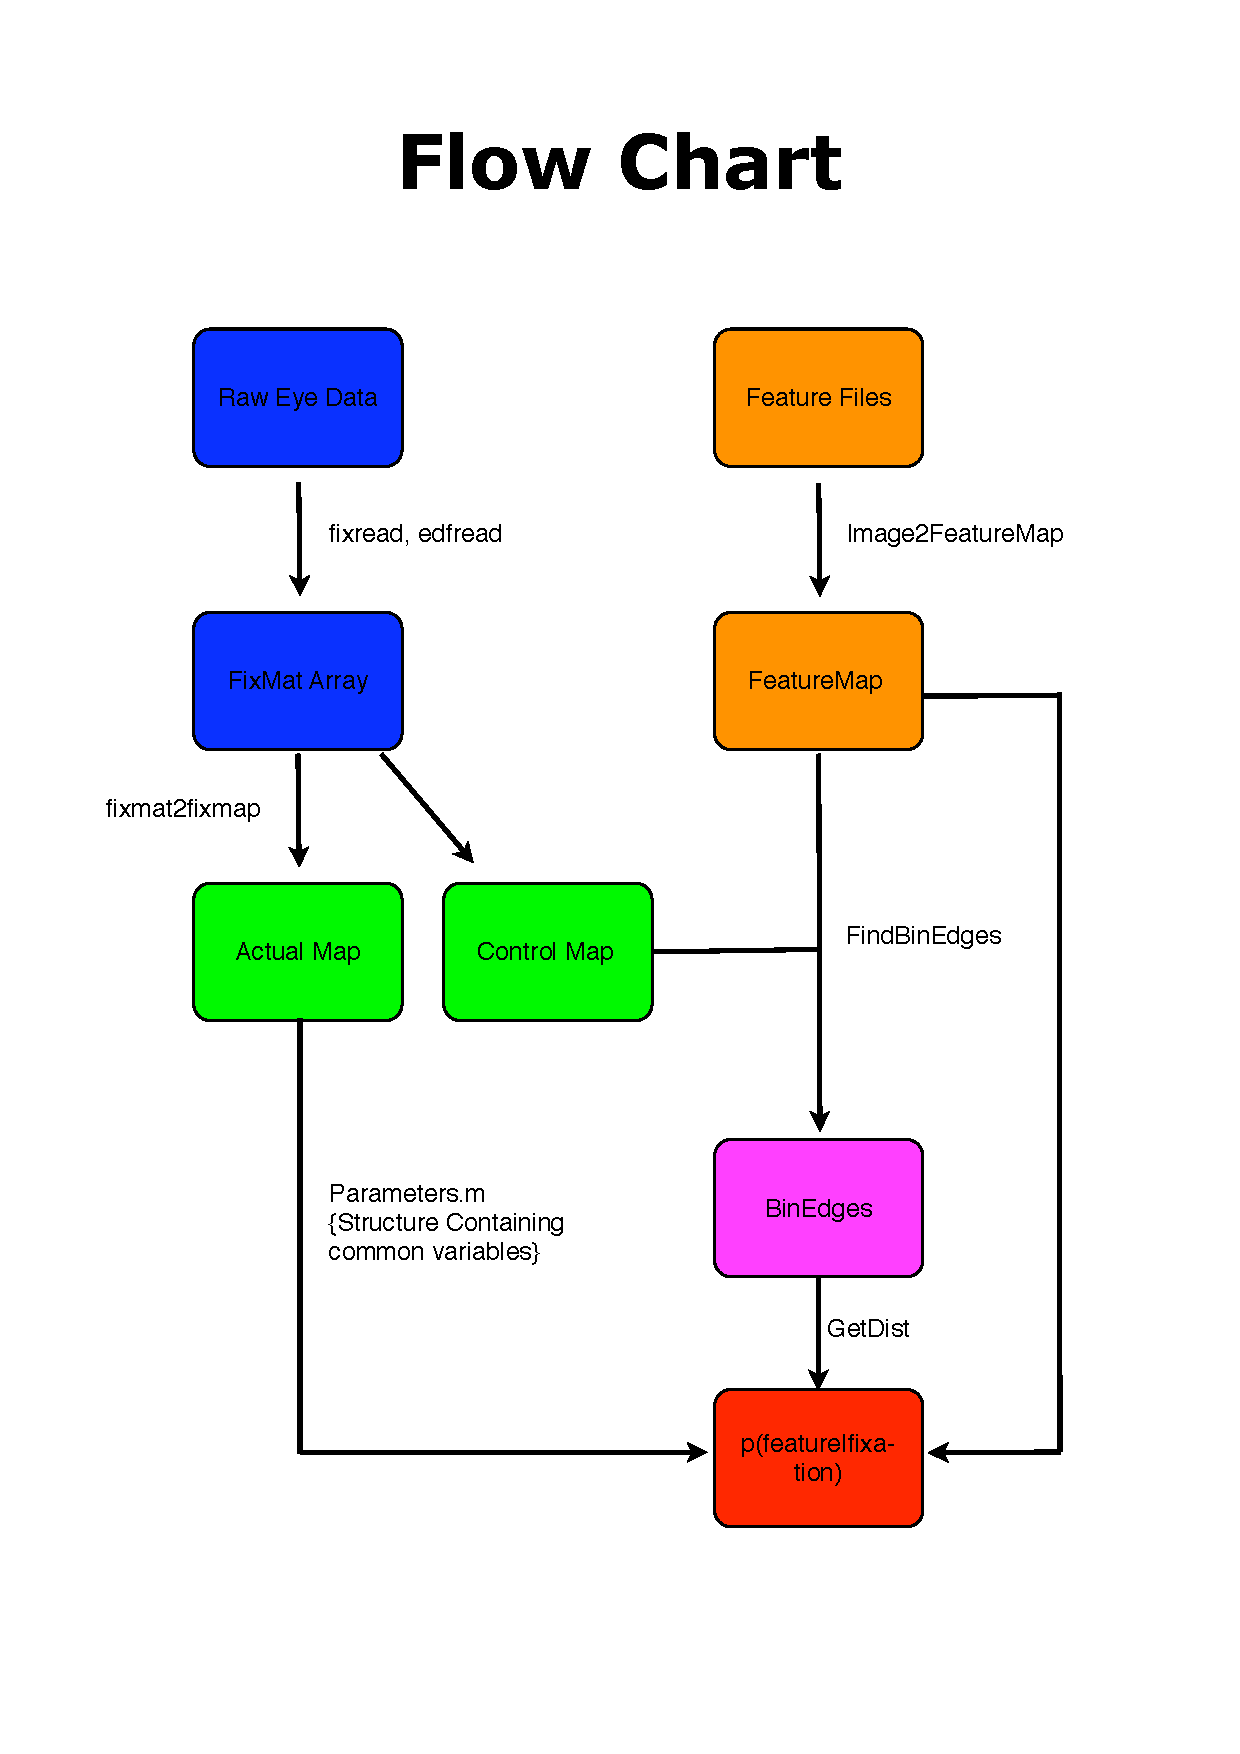
\includegraphics[width=8cm]{FlowChart.pdf}
\end{figure}

\section{General Requirements}

You need to respect to some folder naming conventions in order to use the toolbox without much problems. The folders you must have created before using the toolbox are listed below. It is recommendede that you first create a project folder (\$) where all the following folders will be stored.
\begin{description}
 
\item[\$/FeatureMaps]

In this folder, feature maps of different images must be stored. Each feature map, such as luminance contrast maps, mean luminance maps etc. must have their own folders. Here is an example of FeatureMap folder organization. 

\hspace{2cm}
\begin{scriptsize}

drwxr-xr-x 2 sonat ustaff 8192 2007-06-01 20:44 RG

drwxr-xr-x 2 sonat ustaff 8192 2007-06-02 02:18 RG\_C\_Radius\_23 

drwxr-xr-x 2 sonat ustaff 8192 2007-06-01 23:08 RG\_C\_Radius\_45

drwxr-xr-x 2 sonat ustaff 8192 2007-06-02 01:28 RG\_M\_Radius\_23

drwxr-xr-x 2 sonat ustaff 8192 2007-06-02 00:18 RG\_M\_Radius\_45

drwxr-xr-x 2 sonat ustaff 8192 2007-06-01 20:44 SAT

drwxr-xr-x 2 sonat ustaff 8192 2007-06-02 03:02 SAT\_C\_Radius\_23

drwxr-xr-x 2 sonat ustaff 8192 2007-06-01 23:03 SAT\_C\_Radius\_45

drwxr-xr-x 2 sonat ustaff 8192 2007-06-02 01:56 SAT\_M\_Radius\_23

drwxr-xr-x 2 sonat ustaff 8192 2007-06-02 00:23 SAT\_M\_Radius\_45

drwxr-xr-x 2 sonat ustaff 8192 2007-06-01 20:44 YB

drwxr-xr-x 2 sonat ustaff 8192 2007-06-02 03:46 YB\_C\_Radius\_23

drwxr-xr-x 2 sonat ustaff 8192 2007-06-02 00:08 YB\_C\_Radius\_45

drwxr-xr-x 2 sonat ustaff 8192 2007-06-02 02:23 YB\_M\_Radius\_23

drwxr-xr-x 2 sonat ustaff 8192 2007-06-02 01:05 YB\_M\_Radius\_45
\end{scriptsize}

\hspace{2cm}

Notice that RG (red-green), SAT (saturation) and YB (yellow-blue) are base features, these are actually different channels of the stimuli. The remaining folders are the feature maps, for example the folder YB\_C\_Radius\_23 contains features maps that represents the Contrast within local patches of 23 pixels for each single image found in YB. Similarly RG\_M\_Radius\_45 contains feature maps that represents the average intensitiy of reg-green channel within patches of 45 pixels.

Within each of the feature folders featuremaps of each stimulus image must be stored as a single \texttt{.mat} file. An example and prefered organization is the following:

\hspace{2cm}

\begin{scriptsize}
-rw-r--r-- 1 sonat ustaff 8904993 2007-06-10 21:09 image\_001.mat

-rw-r--r-- 1 sonat ustaff 8912429 2007-06-10 21:09 image\_002.mat

-rw-r--r-- 1 sonat ustaff 8900295 2007-06-10 21:09 image\_003.mat

-rw-r--r-- 1 sonat ustaff 8910572 2007-06-10 21:09 image\_004.mat

-rw-r--r-- 1 sonat ustaff 8945344 2007-06-10 21:09 image\_005.mat
.

.

.

-rw-r--r-- 1 sonat ustaff 8898754 2007-06-10 21:26 image\_254.mat

-rw-r--r-- 1 sonat ustaff 8896367 2007-06-10 21:26 image\_255.mat
\end{scriptsize}

\hspace{2cm}

Note that there is no distinction concerning the conditions on the filenames, this information is contained either in the input arguments to the toolbox, or alternatively you may want to create different folders for different conditions (however in this latter case, mind that the feature percentiles will be computed separately for each folder, so if you separate conditions into different folders the feature percentiles will be computed separately). 

\item[\$/BinEdges] 

Within this folder bin edges will be stored as \texttt{.mat} files. (If you dont know what it are 'bin edges', there are many sources on the References section). Each bin edges data will have a unique filename specifying the parameters that were used during its computation. If you would like to compute bin edges of the Luminance Contrast features, of a given condition with a given smoothening factor, within the first half of the presentation etc. etc. all this will be stored on the filename, thus leading to somewhat strange filenames. However these filenames will be very handy when we would like to know the parameters a given bin edges has been computed with.

\item[\$/PostDist]
By using each bin edge file and its corresponding feature map we compute the Posterior probabilities (that is probability of fixation given a feature value or feature percentile). These are stored in this folder. Filenames within this directory are exactly the same as the filenames within the BinEdges folder.

\end{description}

Except the featuremap folder, users do not need to actively maintain the \$/BinEdges and \$/PostDist folders. Because the content of these folders are created by functions which know how to choose their filenames. However you have to take that everything is perfectly fine within the \$/FeatureMap directory. That is all the folders dedicated to different features in \$/FeatureMap must have the same naming conventions, and there must be no images missing etc.

The toolbox relies exclusively on the usage of the standard \textit{fixmat} format to make anything meaningful with the fixation data. However you must add to the fixmat a field called \texttt{.rect} containing the size of the images shown. In case your images are 960 times 1280, then you would need to add the \texttt{.rect} field in the following way: 

fixmat.rect = [0 960 0 1280] 

An example fixmat structure is included in the toolbox, you will need to adapt your own fixation points to this format.


\section{List of Basic Functions}
Here you find a short description of what the functions are doing. More help is available on their help section, just type \texttt{help \{functionname\}} in matlab command line.

\subsection{Feature Map Related Functions}

These functions computes the \textit{contrast} and \textit{mean} maps of the stimulus i.e. different images. They save their results in specific folders which have their unique names formed according to their input arguments. You may use these functions together with different \textit{base features}. For example if you would like to compute the \textit{luminance contrast map} of a set of images you would need to run \texttt{GetContrastMaps} function on the Luminance base feature. Luminance base feature is nothing but the luminance values of the images. You may, by using the same function compute the \textit{red-green color contrast} of a set of images by using red-green base feature. Depending on what you feed to these functions they produce different feature maps but the underlying computations are the same.

\begin{itemize}
\item \texttt{GetMeanMaps(r,varargin)}

Uses \texttt{LuminanceMap2.m}. \texttt{R} is the diamater of the circular (not gaussian) patch. \texttt{VARARGIN} is the name of the feature folder where the mean luminance maps must be computed. For example, below three feature maps are given (these are some of the folders which are located in the \$/FeatureMap folder). 

\$/FeatureMap/LUM             

\$/FeatureMap/LUM\_M\_Radius\_23 

\$/FeatureMap/LUM\_M\_Radius\_45 
		
The folder LUM contains the raw images shown to the subjects during the experiments, that is why it is referred as a \textit{base feature}. 

The function \texttt{GetMeanMaps} when used in the following way

\texttt{>> GetMeanMaps(23,'LUM');}

it loads the images within the directory LUM and computes the mean luminance maps and saves the results in a folder named LUM\_M\_Radius\_23. \_M\_ holds for 'mean'.

\item \texttt{GetContrastMaps(r,varargin)}

Relies on \texttt{ContrastMap2.m}. It is very similar to \texttt{GetMeanMaps} function in the way it operates however instead of measuring the mean luminance maps, it computes the contrast maps (Uses \_C\_ instead of \_M\_ while creating the feature specific folder. Just keep in mind that 

		\texttt{ >> GetContrastMaps(23,'LUM')}

		would compute the contrast maps of the images and save the results in folder LUM\_C\_Radius\_23. A second run of the same function on the resulting folder 

		\texttt{>> GetContrastMaps(120 , 'LUM\_C\_Radius\_23' )}

		would compute the contrast map of the contrast maps stored in folder LUM\_C\_Radius\_23 to the folder LUM\_C\_Radius\_23\_C\_Radius\_120. This is the way how to obtain texture maps.

\end{itemize}

\subsection{Helper Functions}
\begin{itemize}
\item \texttt{FeatMap = Images2FeatMap(path,ImIndex,varargin)]}

It is used to load feature maps to the working space. 

Usage: 

	\texttt{>> Images2FeatMap(['\$/FeatureMaps/' FeatureName ],1:10)} 

With this usage it loads the first 10 images to the memory. It is handy to use this function with \texttt{GetFeatures}
as it provides a easy way to refer to different feature folders.
As a default behavior it opens the individual feature maps as they are stored without any further modification. VARARGIN can be used to specify a given amount (in pixels) to be cropped from the all of the edges. That if varargin is equal to 200, then 200 pixels are cropped, leading a reduction of 400 pixel of size in a given cardinal direction. This is useful when you would like to have all the feature maps you are working on to have the same number of cropping amount independent of the window sizes.


 \item \texttt{[p,a,d]=CircularPatch(r)}

Computes a circular mask. This is used by functions which are responsible of feature map computation.

 \item \texttt{[map,nPix]=CropperCleaner(map,varargin)}

This function is used to remove the zeros of the zero-padding or to crop a specified amount of pixels from the 2D feature maps. Feature maps have always their size smaller then the original images. This is due to the fact that it is not possible to compute the feature values at the edges of the images. That is why they are saved after zero padding with a necessary amount of zeros so that the size of the feature maps matches to the size of the original images. However care must be given so that the zeros values are not used as feature values for computations based on the feature maps. With this function you can easily manipulate the zeros padding. 


 \item \texttt{p = GetParameters}

	This is one of the most important functions. It provides all the parameters that are necessary to make any further computations. It contains the following fields (the values which are shown below are arbitrary): 
	
	\begin{itemize} 	 
		\item \texttt{p.FWHM: 45} 

		This is the Full Width Half Maximum (in pixels) of the gaussian smoothening kernel. To correctly use this you must know how to transform degrees into pixels for your specific setup.
    		\item \texttt{p.CropAmount: 0} 

		This is the number of pixels that a feature map must be cropped from all of its edges. This is necessary to remove the edge artefacts of feature maps. Use this to have all the feature maps to have the same amount.
        	
		\item \texttt{p.kernel: [117x117 double]} 

		This is the smoothening gaussian kernel. It is computed according to the value of the FWHM field.
        	
		\item \texttt{p.nBin: 20} 
		
		Number of bins where the posterior distribution will be computed.

        	\item \texttt{p.start: 0} 
           	
		\item \texttt{p.end: 6500} 

		Start and end values (in ms) determine the interval of the stimulus presentation that must be used for the analysis. For example if it is equal to [ 0 2000] only the fixation within the first 2 seconds are included. This uses the fixmat structure to filter the fixations, therefore mind using the same units.

           	\item \texttt{p.nBS: 0} 
		
		Number of bootstraping.

           	\item \texttt{p.fix: 2} 

		The first valid fixation index. If it is equal to 2, then the first fixation of all trials are excluded from the analysis.

      		\item \texttt{p.subjects: [1 2 3 4 5 6 7 8 9 10 11 12 13 14 15 16 17 18 19 20 21 22 23 24 25]} 

		The indices of the valid subjects, this is in register with the fixmat structure.
        	
		\item \texttt{p.folder: [1x134 char]} 

		This is the tag of the current parameters used. It is unique for this parameter structure array and it will be used to save the derived data such as bin edges and posterior distributions. It is created by calling \texttt{Param2Folder} function.

     		\item \texttt{p.ffcommand: {'fix'  [1x999 double]  'start'  [0]  'end'  [6500]  'subject'  [1x25 double]}} 

		This field will be used in \texttt{GetDist} function. 

	\end{itemize}

This function when used without any input arguments simply returns all the default values. However you may overwrite the default values by entering first the name of the field and second its new value. For example 
	
	\texttt{>> GetParameters('FWHM',90);}
	
would overwrite the FWHM defaults value with the entered value 90. The \texttt{P} structure array will be used ubiquitously during the analysis. It will be passed to many other functions and specify the necessary parameters.

\item \texttt{folder=Param2Folder(p)}

It is used to generate a fingerprint specific to the current state of parameters. Used mainly with \texttt{GetParameters.m}

\item \texttt{f = GetFeatures}

With this function you can easily get a list of feature folder you have. It will be very handy when you will need to enter feature folder names to different functions.
	
	\texttt{>> f = GetFeatures;}  

	Returns all the features you have in your FeatureMap folderas a cell of string arrays.

	\texttt{>> f = GetFeatures('LUM*');}  

	Returns all the features which starts with the string 'LUM'.

\item \texttt{FixMap=fixmat2fixmap(fixmat,kernel,CropAmount,varargin)}

This function is used to create fixation maps. The varargin inputs are passed to \texttt{SelectFix} function.

	\texttt{>> fixmap = fixmat2fixmap(fixmat,p.kernel,0);}

	\texttt{FIXMAP} is the fixation map computed with all of the fixations which is present in \texttt{FIXMAT}. To smoothen the binary map, It uses the kernel contained in \texttt{P} structure array (usually obtained by calling \texttt{GetParameters}). It applies no cropping as the last input is zero.

	\texttt{>> fixmap = fixmat2fixmap(fixmat,p.kernel,100,'image',1:10);}
	Computes a fixation map using images one to 1.

	\texttt{>> fixmap = fixmat2fixmap(fixmat,p.kernel,100,'image',1:10,'fix',2:1000);}
	Computes a fixation map using images 1 to 10 without taking into acount the first fixations.
	\texttt{>> fixmap = fixmat2fixmap(fixmat,1,100,'image',1:10,'fix',2:1000);}
	Computes a non smoothened map as the kernel is simply 1.

\item \texttt{fixmat=GetFixMat(i)}

This function must be adapted according to your setup. It simply load the \texttt{$I^{th}$} fixmat file. If you have more then one fixmat, it is handy to load to the working space the desired fixmat.

\item \texttt{be=Load\_FindBinEdges(feat,cat,p)}

It loads the bin edges \texttt{BE}, computed with the feature \texttt{FEAT}, condition CAT and parameter array \texttt{P}. The bin edges files are written to the disk by the meta function \texttt{All\_FindBinEdges} which calls FindBinEdges.

\item \texttt{[varargout]=SelectFix(fixmat,varargin)}

This is an extremely handy function that is used to filter the fixmat structure array. Example usage:


\texttt{>> fixmat2 = SelectFix(fixmat,'subject',1:10)}

	Removes all the fixations within the fixmat array \texttt{FIXMAT} which do not belong to subjects one to ten. That is all the fixation data in \texttt{FIXMAT2} would be composed of the data originating from subjects one to ten.

\texttt{>> fixmat = SelectFix(fixmat,'fix',2:1000)}

	Remove all the first fixations.

\texttt{>> fixmat = SelectFix(fixmat,'image',1)}

	Keep only the data done on the first image.

\texttt{>> fixmat = SelectFix(fixmat)}

	Calling the function without any other argument then fixmat would simply remove the fixations which are out of the screen.

\end{itemize}

\subsection{Core Functions}

You will not need to use these function directly on the command line. They are called by meta function listed in the next section.
\begin{itemize}
	
\item \texttt{BinEdges=FindBinEdges(FeatureMap,FixMap,nBins)}

This function computes the binedges leading to histogram equalization. That is the occurence of the feature values (after being weighted by the central bias) when counted within the bins detected with this function is equal for all the bins.

\texttt{FEATUREMAP} is the result of \texttt{Images2FeatMap}. \texttt{FIXMAP} is the fixation map, it is the result of \texttt{fixmat2fixmap}. Each computation of bin edges needs a weight matrix because not all part of the monitor
are likely to be seen, this weight matrix represents the central bias of the subjects. \texttt{NBINS} is the total number of bins you would like to devide the feaeture space.
		
Usage:

\texttt{>> p          = GetParameters;} 

Get the default parameter values.

\texttt{>> fixmap     = fixmat2fixmap(fixmat,p.kernel,p.CropAmount);}

Get the control fixation map.

\texttt{>> [BinEdges] = FindBinEdges(f.data,fixmap,20);}

Compute the bin edges.
 
\item \texttt{res = GetDist(fixmat,p,varargin)}	

This is the longest function and it is responsible of generating the posterior probabilities. It is recommended that you understand what is going on inside. It is compatible with N dimensional distributions that is, it can accept any number of binedges and feature maps pairs. It computes for N dimensional feature space the posterior probabilities. It is highly recommended that after you use this function you simply check that your control distributions are flat.

\item \texttt{c=Core(FixMap,varargin)}

You will never need to call this function on the command line, GetDist heavily relies on this function. See help Core for more information.
	
		
\end{itemize}
\subsection{Meta Functions}
\begin{itemize}
	
\item \texttt{All\_FindBinEdges(f,p)]}
This function computes the bin edges for the features in \texttt{F} according to the parameters stored in \texttt{P}. \texttt{F} contains the output of \texttt{ListFiles}. You must use ListFiles function in order to obtain a list (as a cell array) of the features names you would like to carry on the analysis. \texttt{P} is the parameter variable, result of \texttt{GetParameters}. This function must be adapted to your requirements. In the current version, the conditions limits (i.e. the first and last frames belonging to a condition) are hardcoded on the function. This will probably change in future. For the time being you must enter by hand your own image indices by hand. At line ~25 you can see the default condition delimiters: [1 64; 65 128; 129 192; 193 255], this means that the image indices belonging to the first condition are from 1 to 64 and the second condition's images have indices from 65 to 128 and so on. The result are saved in the folder \$/BinEdges.
\item \texttt{[All\_GetDist(FileList)]}

Similar to the previous function, This function computes the posterior probabilities for all the computed bin edges. \texttt{FILELIST} is cell array containing the filenames of different bin edges stored in the folder \texttt{BinEdges}. The results are saved in \$/PostDist folder.
	


\end{itemize}

\subsection{Acknowledgements}

Frank Schumann, Alper Acik, Johannes Steger, 

\subsection{References}

\href{http://www.academia.edu/538828/Integration_of_different_features_in_guiding_eye-movements}{master thesis of Frank Schumann

Ossandon

Onat


\end{document}
